\documentclass[9pt]{template/developercv}
\usepackage[danish]{babel}

% Commands
\newcommand{\nametitlebox}[1]{\colorbox{black}{{\HUGE\textcolor{white}{\textbf{\MakeUppercase{#1}}}}}}
\newcommand{\link}[2]{\faLink~\href{#1}{\textbf{#2}}}

% Settings
\setlength{\tabcolsep}{4pt}

\begin{document}

% HEADER (name, contact information)
% ------------------------------------------------------------------------------
\begin{minipage}[c]{0.7\textwidth}
  \vspace{-\baselineskip}
  \nametitlebox{Janus Sejersbøll}
  \nametitlebox{Valberg-Madsen}

  \vspace{1em}
  {\huge \faGraduationCap\ cand.scient.oecon}
  \vspace{1em}

  \hspace{-4pt}
  \begin{tabular}{lll}
    \icon{Envelope}{10}{\href{mailto:janusvm@pm.me}{janusvm@pm.me}}
    & \icon{Phone}{10}{+45 21 38 81 15}
    & \icon{MapMarker}{10}{DK-9000 Aalborg} \\
    & & \\
    \icon{Github}{10}{\href{https://github.com/janusvm}{github.com/janusvm}}
    & \icon{Gamepad}{10}{\href{https://atokniiro.itch.io}{atokniiro.itch.io}}
    & \icon{Linkedin}{10}{\href{https://www.linkedin.com/in/janusvm}{linkedin.com/in/janusvm}}
  \end{tabular}
\end{minipage}
\begin{minipage}[c]{0.3\textwidth}
  \vspace{-\baselineskip}
  \flushright
  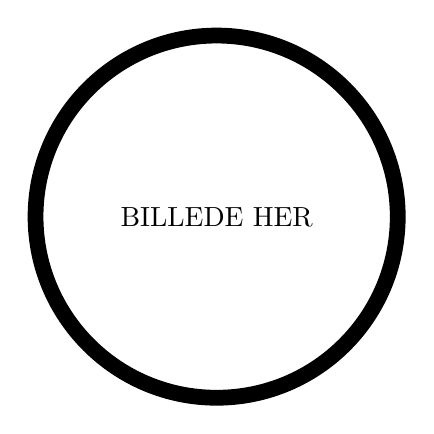
\begin{tikzpicture}
    \node at (0,0) {BILLEDE HER};
    \draw[line width=2mm] (0,0) circle (23mm);
  \end{tikzpicture}
\end{minipage}

\vspace{1em}

% INTRO ------------------------------------------------------------------------
\cvsect{Hvem er jeg?}

\begin{minipage}[t]{0.5\textwidth}
  \vspace{-\baselineskip}

  Kandidat i matematik-økonomi, 28 år, oprindeligt fra Thy og bor nu i Aalborg med min kæreste og vores 2-årige datter.

  \medskip
  Har en analytisk og kritisk tilgang til problemløsning og masser af erfaring med at arbejde effektivt i grupper, undervise og vejlede samt holde præsentationer for kolleger og i interessegrupper.

  \medskip
  Har siden gymnasiet haft en stødt voksende interesse for programmering og holder af at lære nye programmeringssprog og paradigmer.
  Søger en stilling i IT-branchen, hvor jeg kan udbygge min viden og løse interessante og udfordrende problemer.

\end{minipage}
\hfill
% Programming languages
\begin{minipage}[t]{0.23\textwidth}
  \vspace{-\baselineskip}
  \begin{barchart}{2.5}
    \baritem{R}{100}
    \baritem{\LaTeX}{100}
    \baritem{Python}{80}
    \baritem{SQL}{70}
    \baritem{Haskell}{50}
    \baritem{VBA}{50}
    \baritem{Julia}{50}
    \baritem{MATLAB}{40}
  \end{barchart}
\end{minipage}
\hfill
\begin{minipage}[t]{0.17\textwidth}
  \vspace{-\baselineskip}
  \begin{barchart}{2.5}
    \baritem{GDScript}{40}
    \baritem{J}{40}
    \baritem{HTML}{30}
    \baritem{CSS}{25}
    \baritem{C++}{20}
    \baritem{Scheme}{20}
    % \baritem{Nim}{5}
    % \baritem{Rust}{5}
    \baritem{Ruby}{5}
    \baritem{Clojure}{5}
  \end{barchart}
\end{minipage}

% Tools
\begin{center}
  \bubbles{
    2/VS Code,
    3/Vim,
    6.5/Emacs,
    6/git,
    5/Make,
    4/CI\&CD,
    4/Linux,
    3/MS Office
  }
\end{center}

% ERFARING ---------------------------------------------------------------------
\cvsect{Erfaring}
\begin{entrylist}
  \entry
  {9/2019 -- 1/2021\\{\footnotesize afbrudt}}
  {Ph.d.-studerende}
  {Aalborg Universitet}
  {
    Varetog undervisningsopgaver i form af bl.a.\ projektvejledning for førsteårsstuderende og forelæsninger om relationelle databaser.
    Begge dele involverede udarbejdelse af undervisningsmateriale, herunder videomateriale ifm.\ fjernundervisning under COVID-19-restriktioner i 2020.

    Drev forskningsarbejde og holdt oplæg på konferencer i både Danmark og udlandet.

    Deltog i stort COVID-19-relateret forskningsprojekt, der involverede et samarbejde mellem adskillige danske universiteter.
  }

  \entry
  {7/2016 -- 7/2018\\{\footnotesize studiejob}}
  {Udvikler og analytiker}
  {Centrica Energy Trading A/S}
  {
    Assisterede day-ahead/cross border power traders med diverse opgaver, herunder udvikling af dashboards og hjælpeværktøjer, udførelse af dataanalyser, organisering af databaser, osv.
    \\
    \texttt{R / SQL / Python / MS Excel + VBA}
  }
\end{entrylist}

% UDDANNELSE -------------------------------------------------------------------
\cvsect{Uddannelse}
\begin{entrylist}
  \entry {9/2016 -- 9/2019} {Kandidat i Matematik-Økonomi} {Aalborg Universitet} {
    Avancerede emner inden for statistik, økonometri, finansiel matematik og machine learning.\\
    \link{https://github.com/janusvm/masters-thesis}{Speciale ( \faGithub/masters-thesis ):}
    \emph{Vine Copulas for Multivariate Time Series Modelling}% , omhandlede \emph{vine copulas} og deres anvendelser inden for prismodellering på europæiske energimarkeder.
  }
  \entry {9/2013 -- 6/2016} {Bachelor i Matematik-Økonomi} {Aalborg Universitet} {
    Fundamental teori inden for matematisk modellering, herunder sandsynlighedsteori, statistik og tidsrækkeanalyse.
  }
\end{entrylist}

% ANDET INFORMATION ------------------------------------------------------------
\begin{minipage}[t]{0.25\textwidth}
  \vspace{-\baselineskip}

  \cvsect{Sprog}

  \begin{tabular}{ll}
    \textbf{Dansk}   & modersmål \\
    \textbf{Engelsk} & flydende  \\
    \textbf{Tysk}    & grundlæggende
  \end{tabular}
\end{minipage}
\hfill
\begin{minipage}[t]{0.7\textwidth}
  \vspace{-\baselineskip}

  \cvsect{Hobbyer}

  Foruden programmering har jeg altid været meget glad for at tegne tegneserier, og i min fritid arbejder jeg på adskillige igangværende projekter.
  Indtil jeg får bygget mit eget site, kan mine offentligt tilgængelige serier findes på \faLink~\href{https://tapas.io/AtokNiiro/series}{\textbf{tapas.io/AtokNiiro}}
\end{minipage}

\end{document}
